	
	
	\documentclass[a4paper,12pt]{article}
	
	\usepackage{graphicx} % Required for inserting images
	\usepackage{amsmath,amssymb,amsfonts}
	\usepackage{subcaption}
	% -----------------------
	% Package Imports
	% -----------------------
	
	% Set page margins
	\usepackage[a4paper, top=1in, bottom=0.8in, left=1.1in, right=0.8in]{geometry}
	
	% Use Times New Roman font
	\usepackage{times}
	
	% Add page numbering
	\pagestyle{plain}
	
	% Enable graphics inclusion
	\usepackage{graphicx}
	\usepackage{float}
	% Enable code listings
	\usepackage{listings}
	\usepackage{xcolor} % For customizing code colors
	\setlength{\parindent}{0pt}
	
	\begin{document}
			\section{Experiment No. 1}
		
		\section{Experiment Title }
	Observation and Familiarization of various modulation and demodulation kits
		\section{Objective}
		
		The objectives of this lab are as follows:
		\begin{itemize}
			\item To explore the practical implementation and circuit configurations of modulation and
			demodulation kits
			\item To understand the working principles of modulation and demodulation techniques
			
		\end{itemize}
		
		\section{Theory}
		\subsection{Types of Modulation}
		Modulation can be broadly categorized into three types:
		
		\begin{enumerate}
			\item \textbf{Amplitude Modulation (AM)}: The amplitude of the carrier signal is varied in proportion to the message signal. It is widely used in radio broadcasting and analog television transmission.
			\item \textbf{Frequency Modulation (FM)}: The frequency of the carrier signal is varied according to the message signal. It provides better noise immunity and is commonly used in FM radio and television audio signals.
			\item \textbf{Phase Modulation (PM)}: The phase of the carrier signal is varied based on the message signal. It is closely related to FM and is used in digital communication systems.
		\end{enumerate}
		
		\section{Types of Demodulation}
		Demodulation is the process of recovering the original message signal from a modulated carrier. The techniques used for demodulation depend on the type of modulation:
		
		\begin{enumerate}
			\item \textbf{AM Demodulation}: Envelope detectors or synchronous detection methods are used to recover the message signal from an amplitude-modulated waveform.
			\item \textbf{FM Demodulation}: Frequency discriminators or phase-locked loops (PLL) are commonly used for demodulating frequency-modulated signals.
			\item \textbf{PM Demodulation}: Phase detectors or differential techniques help in retrieving the original signal from a phase-modulated wave.
		\end{enumerate}
		
		\section{Frequency Modulator and Demodulator Components}
		
		\textbf{Frequency Modulator:} This circuit varies the frequency of a carrier signal based on the input (message) signal. Key components include:
		\begin{enumerate}
			\item \textbf{Voltage-Controlled Oscillator (VCO):} Generates the carrier whose frequency is tuned by the input voltage.
			\item \textbf{Modulation Circuitry:} Often employs varactor diodes or mixer stages to imprint the message signal onto the carrier.
			\item \textbf{Amplifiers and Filters:} Condition and enhance the modulated signal for transmission.
		\end{enumerate}
		
		\textbf{Frequency Demodulator:} This circuit extracts the original message signal from the frequency modulated carrier. Its main elements are:
		\begin{enumerate}
			\item \textbf{Frequency Discriminator:} Converts frequency variations into corresponding amplitude variations.
			\item \textbf{Phase-Locked Loop (PLL):} Tracks the carrier frequency and generates an error signal proportional to the modulation.
			\item \textbf{Filtering Network:} Removes unwanted noise to recover a clean baseband signal.
		\end{enumerate}
		
		
		
		\section{Trainer Kit list }
		\begin{enumerate}
					\item	Integrated AM-FM Radio Trainer Base Station.
			\item   LCD/LED TV Trainer
			\item	Amplitude modulation transmitter kit
			\item	Amplitude Demodulator Receiver kit
			\item	Frequency (FM) demodulation receiver kit
			\item	Frequency (FM) Demodulation receiver kit
			\item	KL-93063 FM transmitter kit
			\item	KL-93062 AM Transistorizen Radio
			\item	KL-93064 STEREO RADIO
			\item	DL 2402 Colour TV Trainer
		\end{enumerate}

		\section{Trainer Kit Descriptions}
		
		\begin{enumerate}
			\item \textbf{Integrated AM-FM Radio Trainer Base Station:} A comprehensive base station that combines both AM and FM radio training, allowing users to experiment with modulation and demodulation techniques.
			\begin{figure}[H]
				\centering
				\includegraphics[width=.7\linewidth, height=0.3\textheight]{"../../../../WhatsApp Image 2025-02-23 at 4.22.25 AM (1)"}
				\caption{Integrated AM-FM Radio Trainer Base Station}
				
			\end{figure}
			
			\item \textbf{LCD/LED TV Trainer:} A trainer kit designed to demonstrate television principles, featuring both LCD and LED display technologies for modern TV system simulation.
			\begin{figure}[H]
				\centering
				\includegraphics[width=0.7\linewidth]{"../../../../2"}
				\caption{LCD/LED TV Trainer}
				
			\end{figure}
			
			
			
			
			
			\item \textbf{Amplitude Modulation Transmitter Kit:} This kit enables learners to build an AM transmitter circuit, illustrating how the amplitude of a carrier is varied by the message signal.
			
			\begin{figure}[H]
				\centering
				\rotatebox{270}{		\includegraphics[width=.5\linewidth, height=0.45\textheight]{"../../../../3"}}
				\caption{Amplitude Modulation transmitter kit}
				
			\end{figure}
			
			
			
			\item \textbf{Amplitude Demodulator Receiver Kit:} A practical kit focused on recovering the original audio signal from an AM waveform using envelope or synchronous detection methods.
				\begin{figure}[H]
				\centering
				\includegraphics[width=.7\linewidth, height=0.3\textheight]{"../../../../4"}
				\caption{Amplitude Demodulator Receiver kit}
				
			\end{figure}
			
			
			
			
			
			
			\item \textbf{Frequency (FM) Demodulation Receiver Kit:} A kit that demonstrates FM signal reception and demodulation, using frequency discriminators or PLL techniques to extract the message signal.
			\begin{figure}[H]
				\centering
				\includegraphics[width=.7\linewidth, height=0.3\textheight]{"../../../../5"}
				\caption{Frequency (FM) Modulation transmitter kit}
				
			\end{figure}
			
			
			
			
			
			
			
			
			
			
			\item \textbf{Frequency (FM) Demodulation Receiver Kit:} (Alternate version) A similar FM receiver kit that may offer additional features or enhancements for exploring FM demodulation.
				\begin{figure}[H]
				\centering
				\includegraphics[width=.7\linewidth, height=0.3\textheight]{"../../../../6"}
				\caption{Frequency (FM) Demodulation receiver kit}
				
			\end{figure}
			
			
			
			
			
			
			
			
			
			\item \textbf{KL-93063 FM Transmitter Kit:} A dedicated FM transmitter trainer (model KL-93063) that provides hands-on experience in constructing and testing FM transmission circuits.
			
			\begin{figure}[H]
				\centering
				\includegraphics[width=.7\linewidth, height=0.3\textheight]{"../../../../7"}
				\caption{KL-93063 FM transmitter kit}
				
			\end{figure}
			
			
			
			
			
			
			
			
			
			
			
			
			\item \textbf{KL-93062 AM Transistorized Radio:} A transistorized AM radio kit (model KL-93062) designed for practical learning in AM radio circuit design and transistor applications.
			\begin{figure}[H]
				\centering
				\includegraphics[width=.7\linewidth, height=0.3\textheight]{"../../../../8"}
				\caption{KL-93062 AM Transistorizen Radio}
				
			\end{figure}
			
			
			
			
			
			
			
			
			
			
			
			\item \textbf{KL-93064 Stereo Radio:} A stereo radio trainer kit (model KL-93064) that demonstrates advanced audio processing and stereo reception principles.
				\begin{figure}[H]
				\centering
				\includegraphics[width=.7\linewidth, height=0.3\textheight]{"../../../../9"}
				\caption{KL-93064 STEREO RADIO}
				
			\end{figure}
			
			
			
			
			
			
			
			\item \textbf{DL 2402 Colour TV Trainer:} A colour television trainer (model DL 2402) used to illustrate the fundamentals of colour TV signal processing and display technologies.
		\end{enumerate}
			\begin{figure}[H]
			\centering
			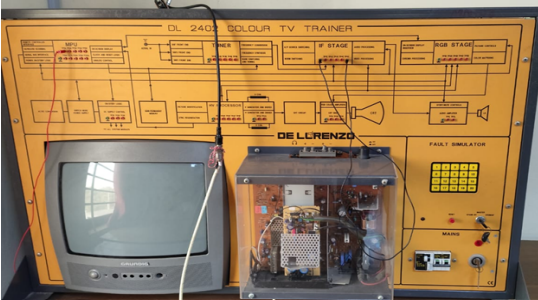
\includegraphics[width=.8\linewidth, height=0.3\textheight]{screenshot001}
			\caption{DL 2402 Colour TV Trainer}
			
		\end{figure}

\section{Discussion}
Various modulation and demodulation kits were introduced to illustrate the principles of amplitude modulation (AM) and frequency modulation (FM). The AM kit was introduced to demonstrate the variation of carrier amplitude by the message signal, while the FM kit was used to show that frequency deviations improved noise immunity. Original message signals were recovered via an envelope detector in the AM demodulator and a frequency discriminator in the FM Demodulator. A comprehensive understanding of these processes was achieved and the usages of the kits were familiarized.


	
	
		
	
		
		
		
		
	
		
		
		
		
		
		
		
	
		
	
		
		
		
		
		
		
	
	\end{document}
	
